\subsection{Iteration \#4}
I iteration 4 ønskes det at udvide systemet med anti kollision. Inden tilføjelsen af anti kollision kan dronen udelukkende flyve i områder uden forhindringer. Men med tilføjelsen af anti kollision vil det være muligt at flyve med dronen i normale områder med diverse forhindringer. 


\subsubsection*{User story}
Under flyvning kontrolleres det løbende hvorvidt der er et objekt foran dronen. Hvis der detekteres et objekt foran dronen, skal dronen holde om med at flyve fremad. I stedet skal dronen dreje horisontalt indtil der ikke længere er et objekt foran den. Når der er frit foran dronen fortsættes den afbrudte flyvning. 
Bruger af systemet har ingen direkte kontakt med anti kollisionssystemet. For bruger ses anti kollision blot som en feature, som gør dronen i stand til at flyve uden at kollidere med objekter foran sig.
 
%kommentar
\begin{figure}[H]
	\centering
	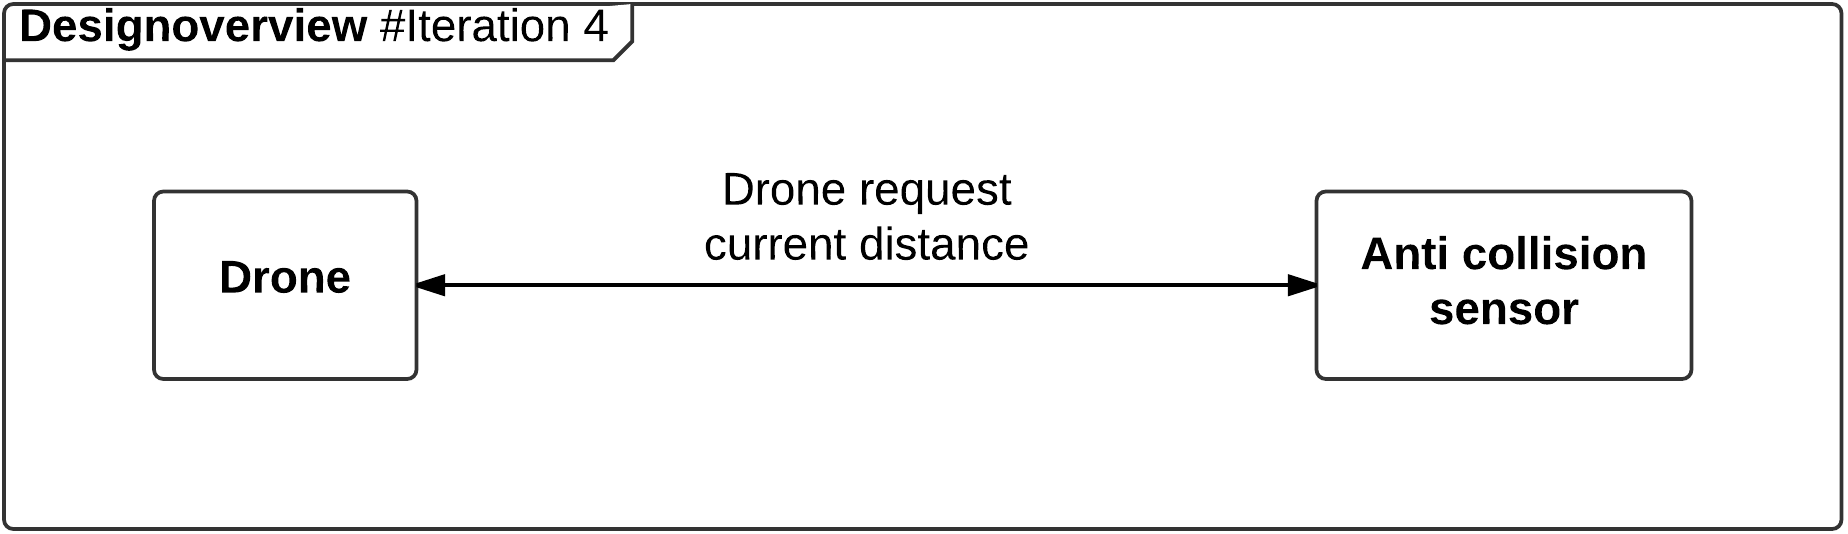
\includegraphics[width=1\textwidth]{Billeder/design_overview/design_overview_iteration4.png}
	\vspace{-.5cm}
	\caption{Designoverview \#iteration 4}
	\label{fig:design_overview_UC4}
\end{figure}

\newpage

\subsubsection*{Pakkediagram drone}
I dette afsnit vises pakkediagram tilhørende drone. Hver pakke i pakkediagrammet består af en eller flere klasser, der med stort samspil udfører opgaver indenfor et fælles ansvarsområde. På hver pakke findes en lille beskrivelse, der tydeliggør pakkens ansvarsområde. 


\begin{figure}[H]
	\centering
	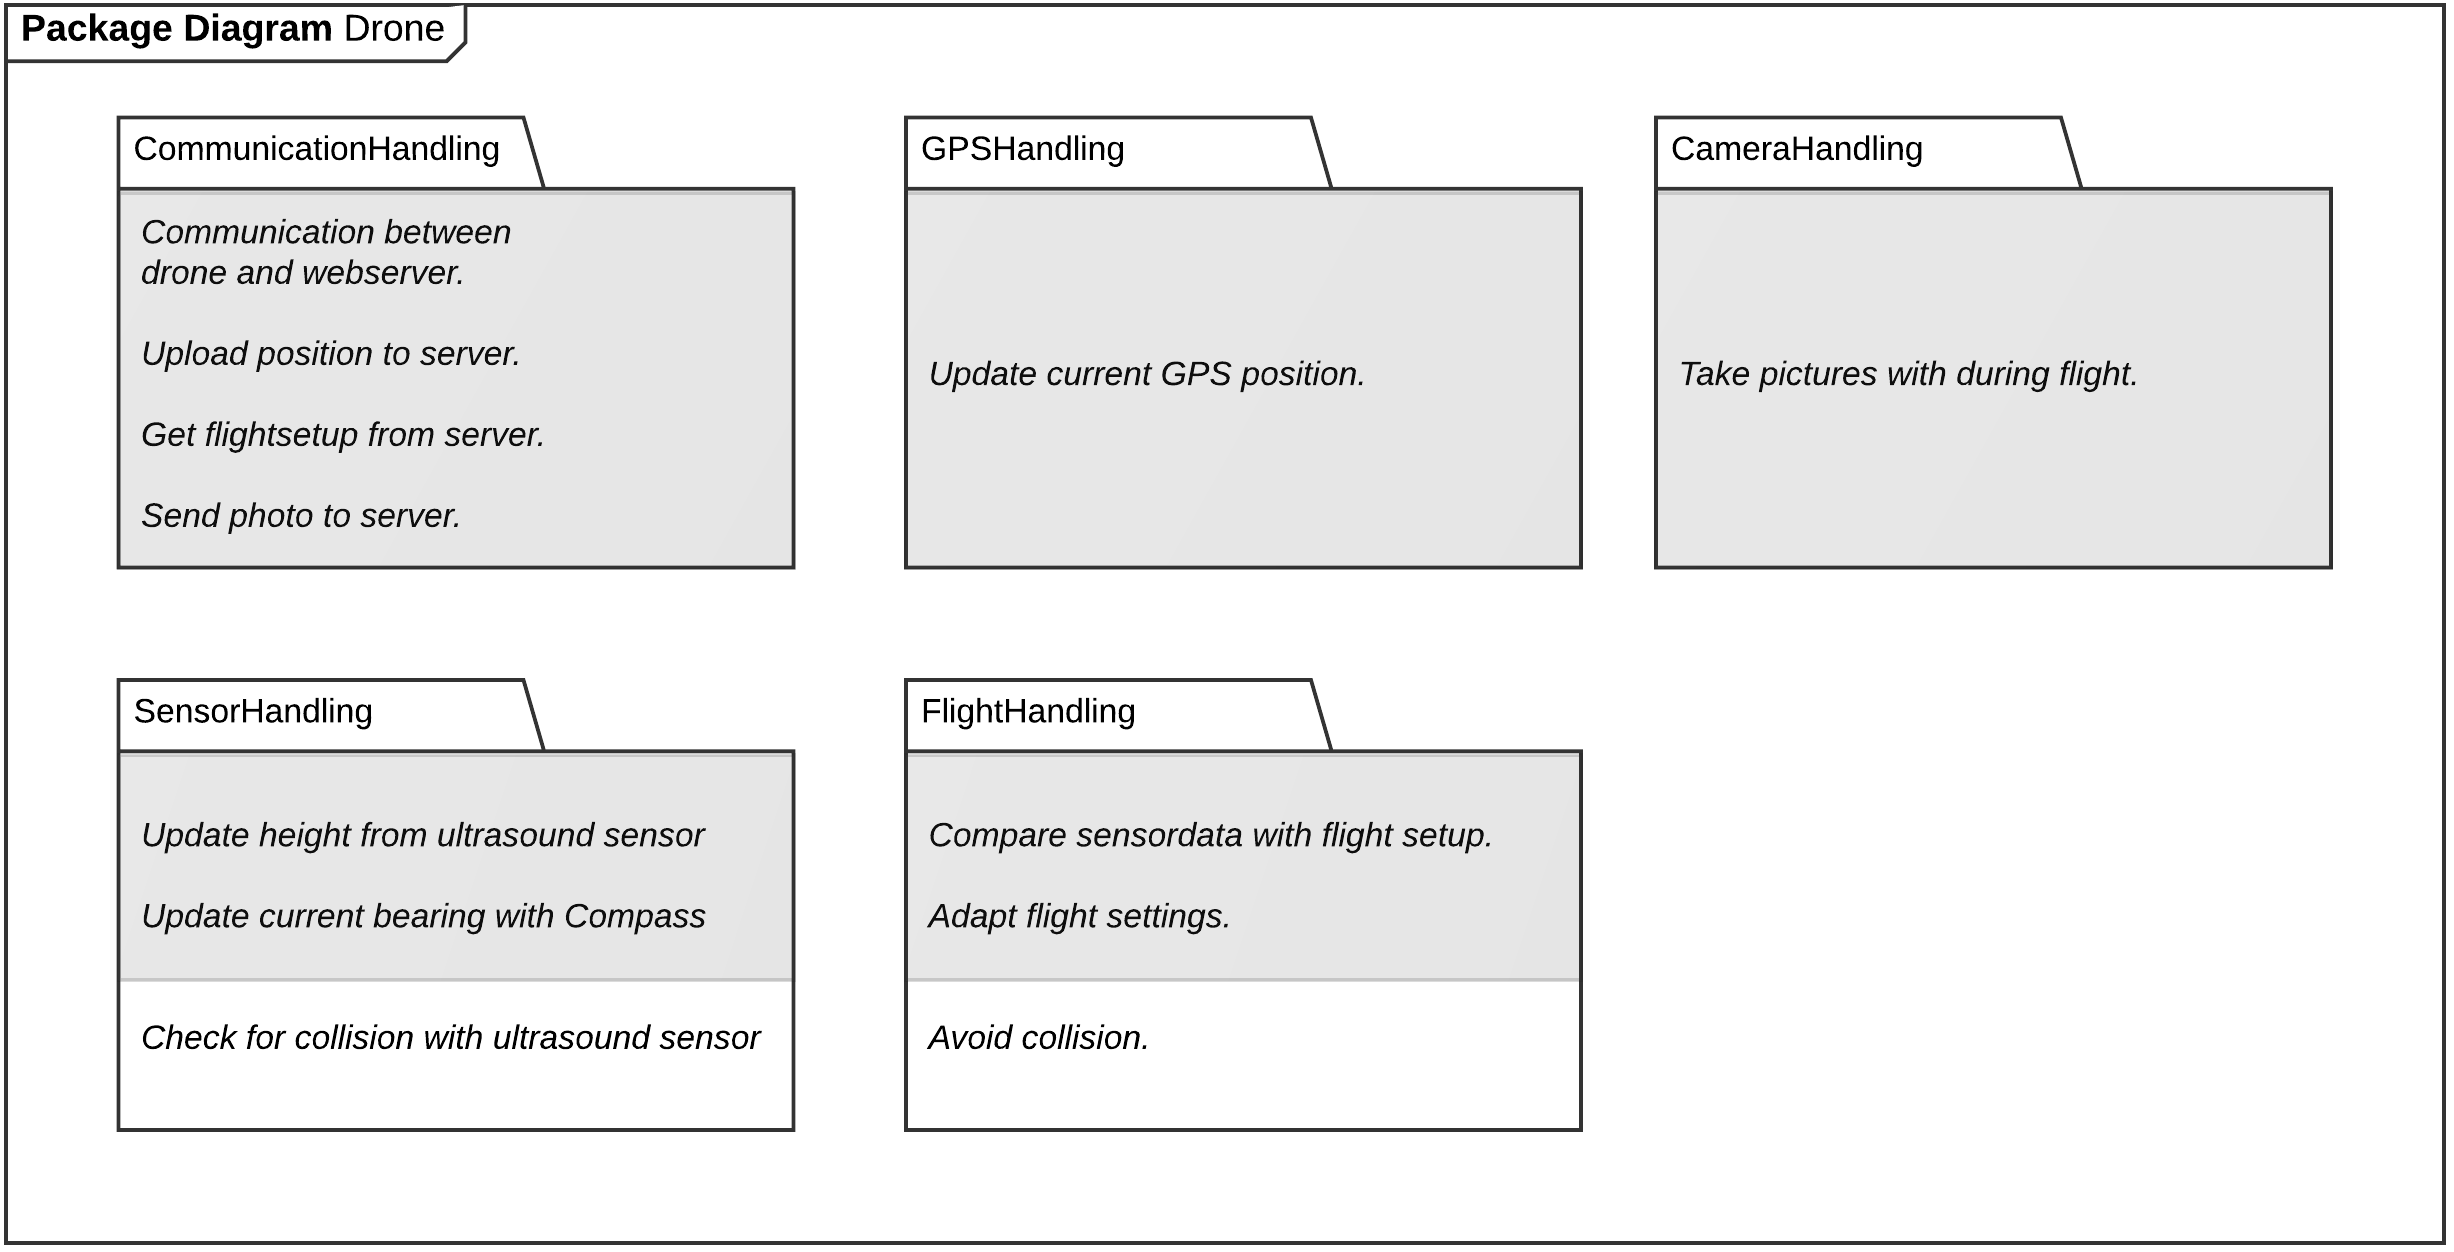
\includegraphics[width=1\textwidth]{Billeder/pakke_diagrammer/iteration4_drone.png}
	\vspace{-0.5cm}
	\caption{Pakkediagram drone}
	\label{fig:iteration4_pakke_diagram_drone}
\end{figure}

\textbf{SensorHandling}\\
Pakken er ansvarlig for indsamling af sensor data. I denne iteration skal pakken bruges til aflæsning af højdemåler, kompas fra flight control boardet og anti kollision sensor. 

\textbf{FlightHandling}\\
Pakkens ansvar er kontrol og styring af drone under flyvning. Ved sammenligning af sensor data og data fra flyveopsætning tilpasses flyvehøjde, orientering mm. 
I denne iteration tilføjes funktionalitet som skal få dronen til at undgå kollision. 

\textbf{GPSHandling}\\
Pakkens ansvar er håndtering af GPS. Dels er pakken ansvarlig for opstart og initiering af GPS. Pakken bruges hver gang dronens nuværende GPS position skal opdateres.

\textbf{CommunicationHandling}\\
Pakkens ansvar er kommunikation imellem drone og server. Efter denne iteration skal dronen kunne hente flyveopsætninger fra server, sende sin nuværende GPS position til server og sende billeder til server.

\textbf{CameraHandling}\\
Pakkens ansvar er håndtering af kamera. Pakken bruges til at starte, initierer, bruge og slukke kameraet.


\newpage
\subsubsection*{Sekvens diagram}
\vspace{-0.2cm}
På sekvensdiagrammet vises de klasser der indgår og bruges i fjerde iteration. 
På diagrammet vises det hvordan afstanden til eventuelle objekter foran dronen kontrolleres. Hvis afstanden til et objekt er under den definerede kollisionsgrænse stoppes dronens fremdrift og der ændres orientering. 


%kommentar
\begin{figure}[H]
	\centering
	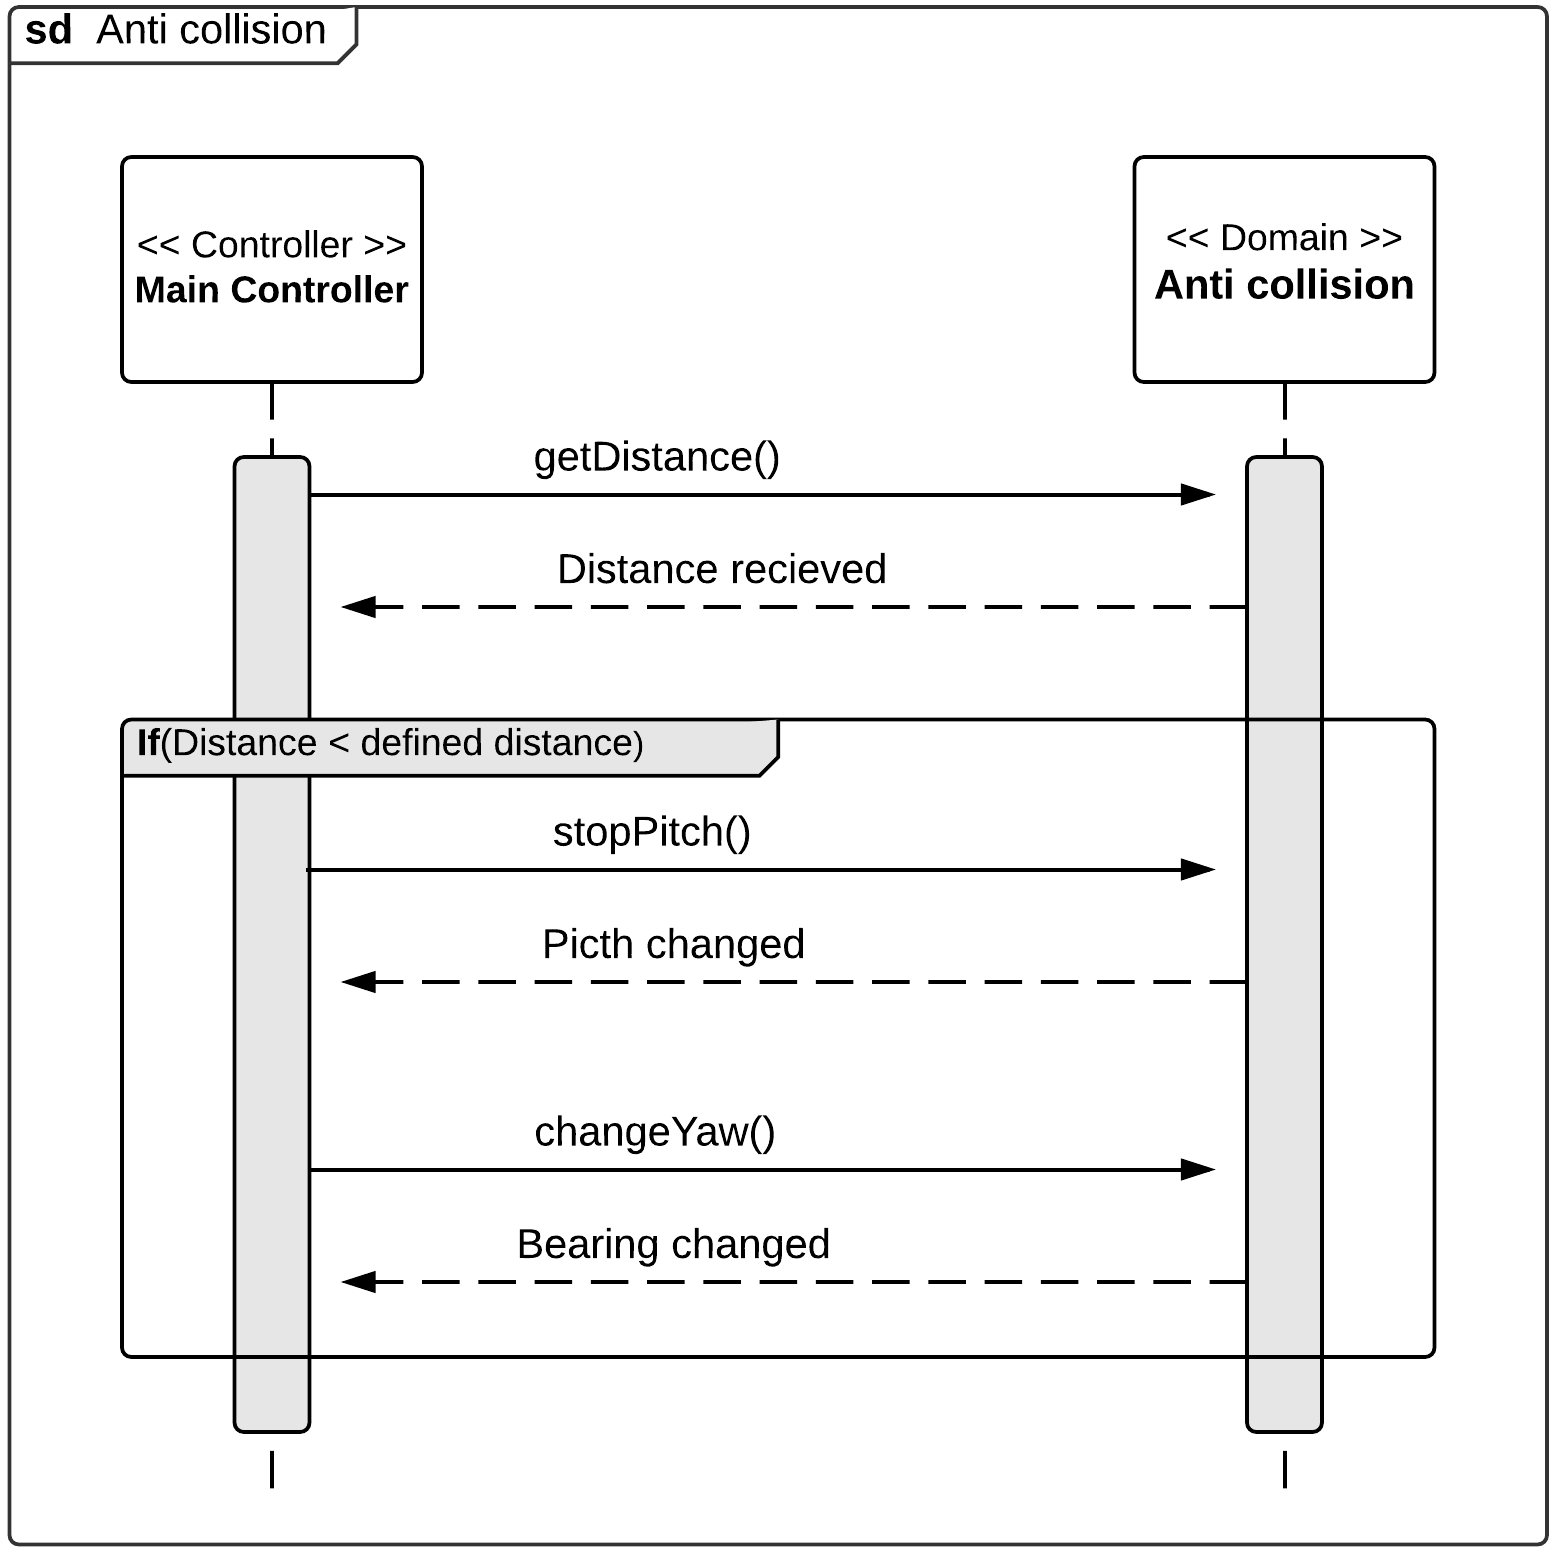
\includegraphics[width=1\textwidth]{Billeder/sekvens/sekvens_iteration4}
	\caption{Sekvens diagram \#iteration 4}
	\label{fig:Sekvens_diagram_iteration4}
\end{figure}


\subsubsection*{Klassediagram drone}
\vspace{-0.1cm}

%kommentar
\begin{figure}[H]
	\centering
	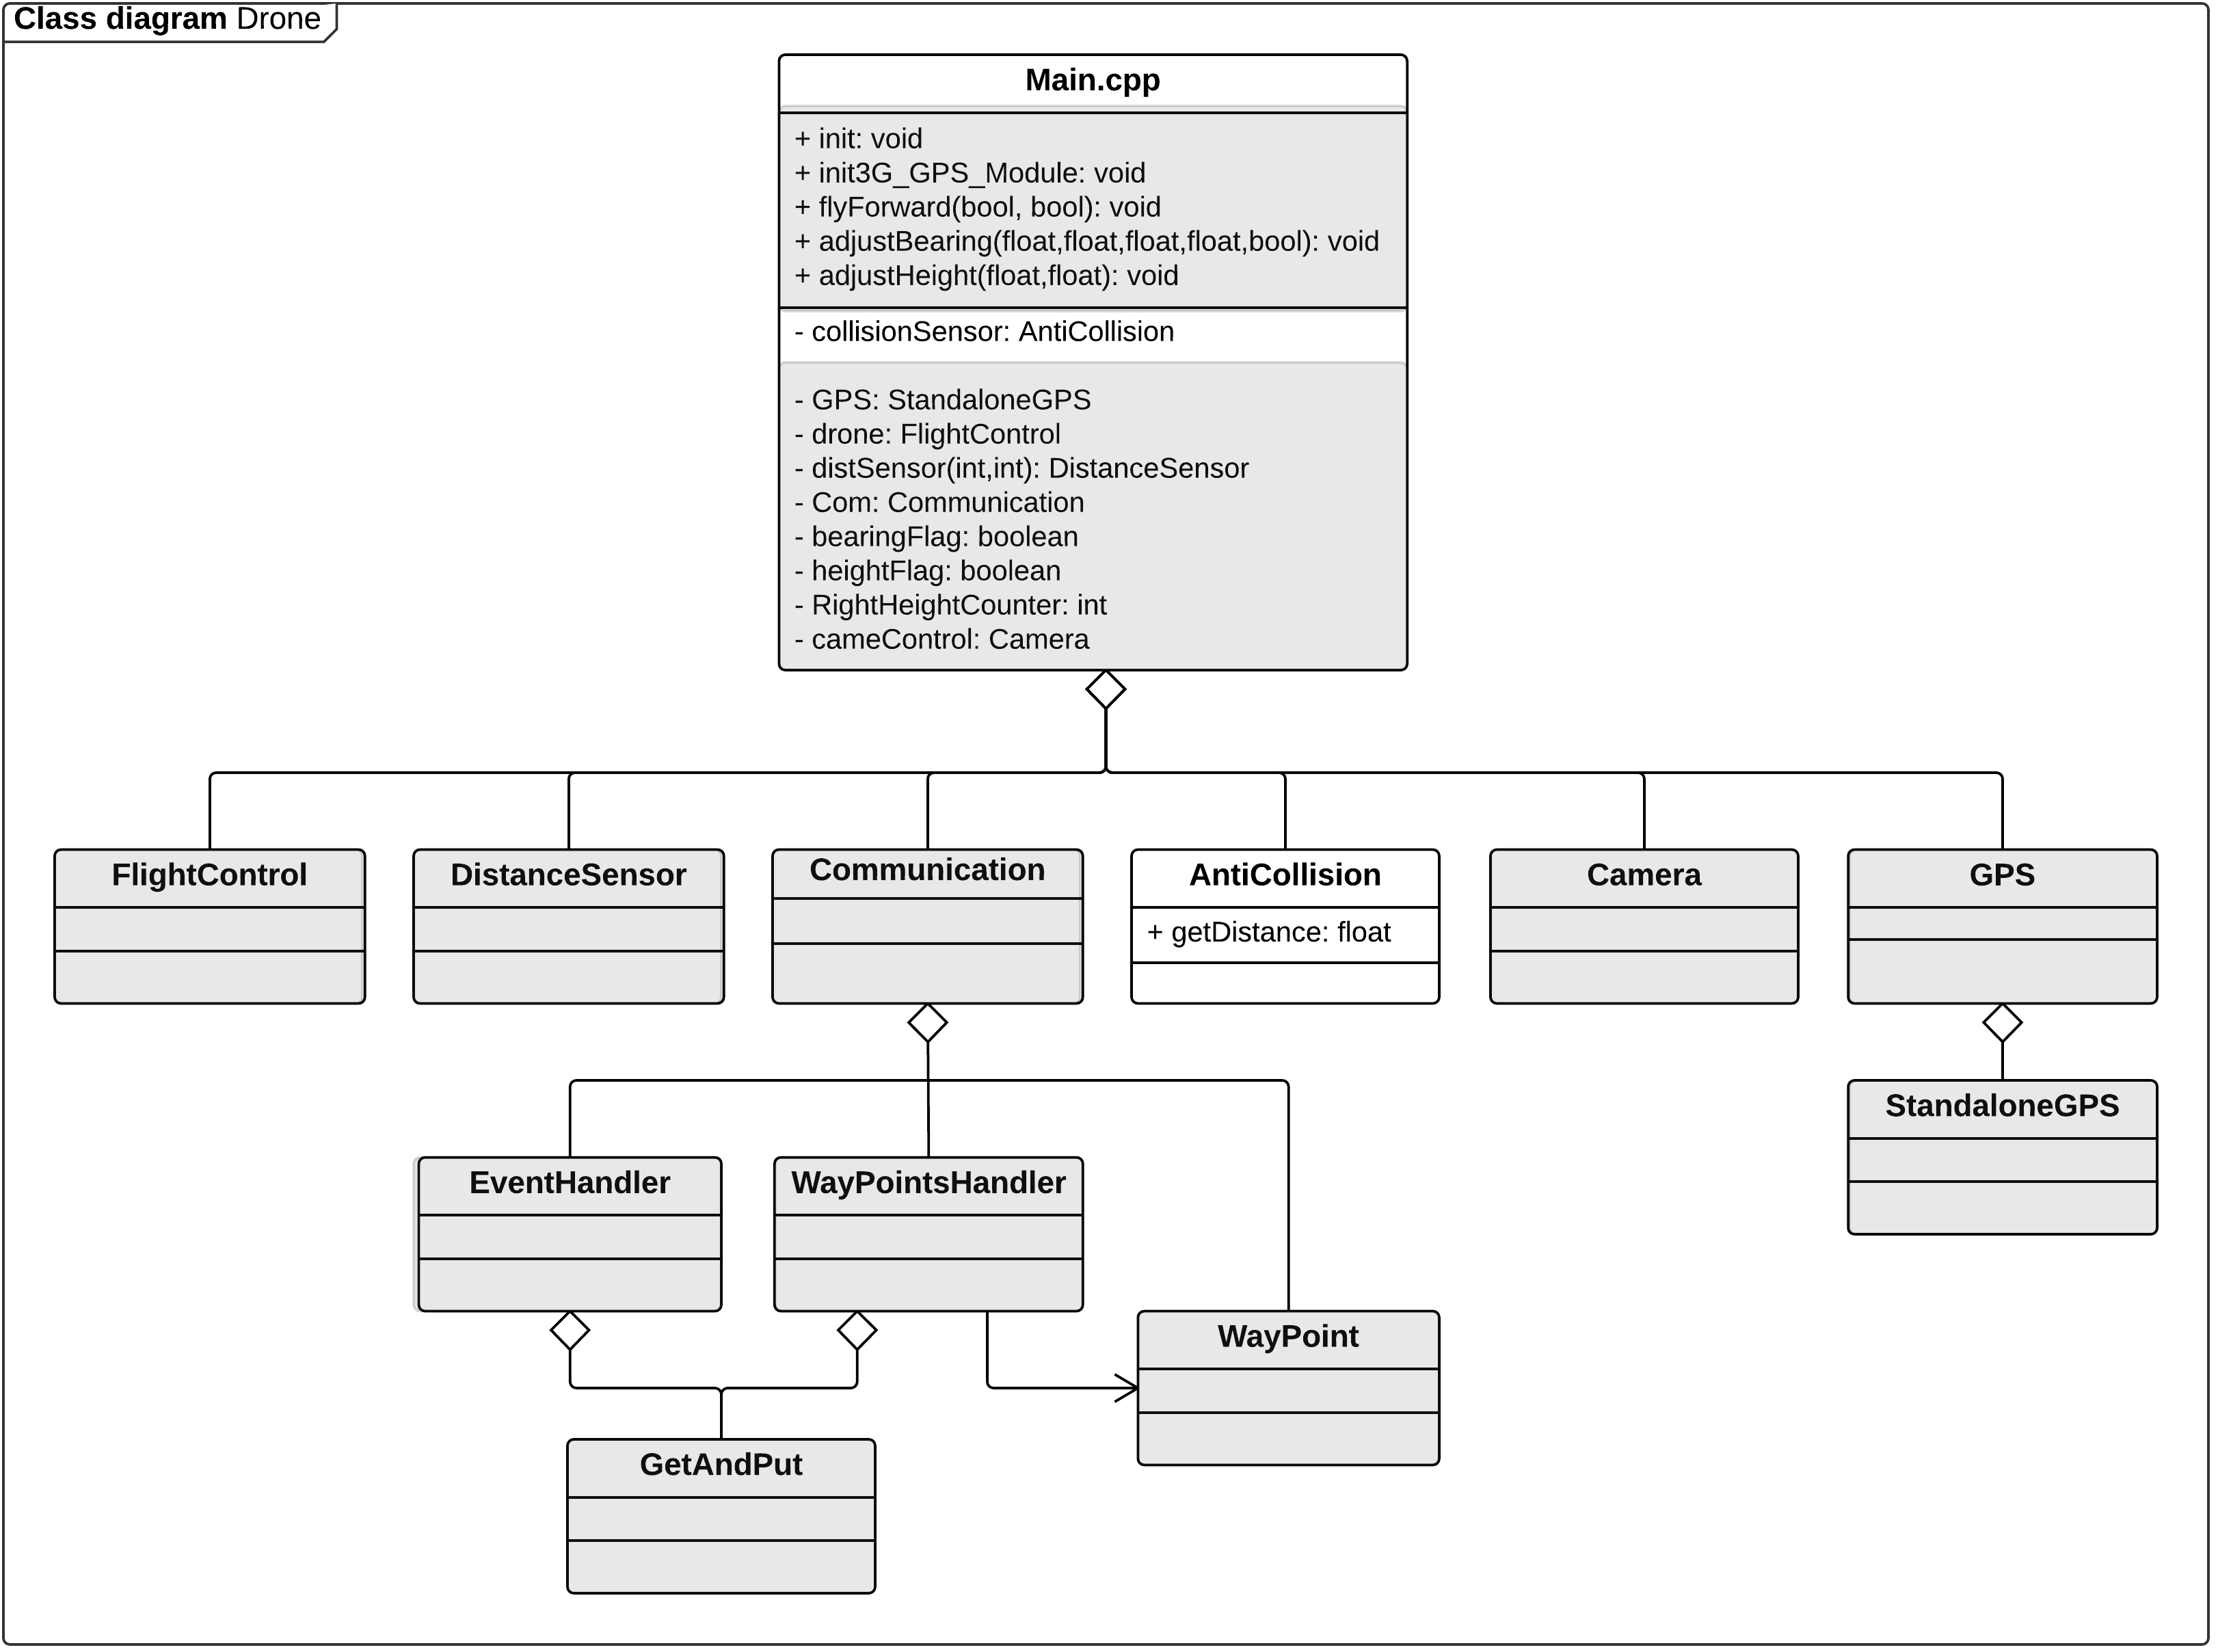
\includegraphics[width=1\textwidth]{Billeder/klasse_diagrammer/classdiagram_iteration4_drone.png}
	\vspace{-0.5cm}
	\caption{Klasse diagram \#iteration 4}
	\label{fig:classDiagram_iteration4}
\end{figure}


\textbf{AntiCollision} \\
AntiCollision klassen fungerer ligesom DistanceSensor. Klassen bruges dog til at kontrollere anti kollisions sensorer der er monteret på dronen. 

\textbf{Camera} \\
Camera klassen er ansvarlig for at tage billeder og sende dem videre i systemet. 

\textbf{FlightControl} \\
FlightControl klassen står for alt styring af dronen. Bla. står FlightControl for kalibrering og styring af motorerne, samt aflæsning af højdesensor, GPS og kompas. 

\textbf{DistanceSensor} \\
DistanceSensor klassen bruges til at kontrollere de sensorer der er monteret på dronen. DistanceSensor klassen bruges udelukkende til kontrol af sensore til højdemåling. 

\textbf{WayPointsHandler} \\
WayPointsHandler klassen håndterer de waypoints der hentes ned fra server. Klassen tager de hentede waypoints og gør dem tilgængelige for main.cpp. WayPointsHandleren gør brug af set-metoder fra WayPoint klassen.

\textbf{WayPoint} \\
WayPoint klassen bruges til at hente waypoints.  

\textbf{Main.cpp} \\
Main.cpp filen bruges til at sætte arduino board korrekt op, bla. sættes baudrate på de forskellige serielle forbindelser. Desuden bruges Main.cpp til at kalde og eksekverer forskellige klasse, objekter og funktioner.

\textbf{GPS} \\
GPS klassen er implementeret som en abstract klasse. Init og updateGPSPosition er lavet som virtuelle metoder, hvilket betyder de skal implementeres i alle afledte klasser. GPS klassen er lavet fordi 3G/GPS modulet kunne bruges i 3 forskellige GPS modes. 

\textbf{StandaloneGPS}\\
Denne klasse er ansvarlig for al kommunikation med GPS'en når standalone mode er valgt. 

\textbf{GetAndPut} \\
GetAndPut klassen er den klasse der er tættest på hardwaren. Klassen indeholder http metoder der bruges til kommunikation mellem dronen og serveren. 

\textbf{Communication} \\
Communication klassen styrer alt der har med 3G kommunikation at gøre.

\textbf{EventHandler} \\
EventHandler klassen håndterer Events, og bruges som bindeled mellem communication- og GetAndPut klassen. EventHandleren sorterer eventID'et fra data der modtages og returnerer værdien af eventID til communication klassen. 

\newpage

\subsubsection*{State machine diagram}
\vspace{-0.2cm}

I state machine diagrammet på figur \ref{fig:Statemachine_iteration4}, vises de states der eksisterer i iteration 4. Desuden vises hvordan flowet imellem de to states ser ud.


%kommentar
\begin{figure}[H]
	\centering
	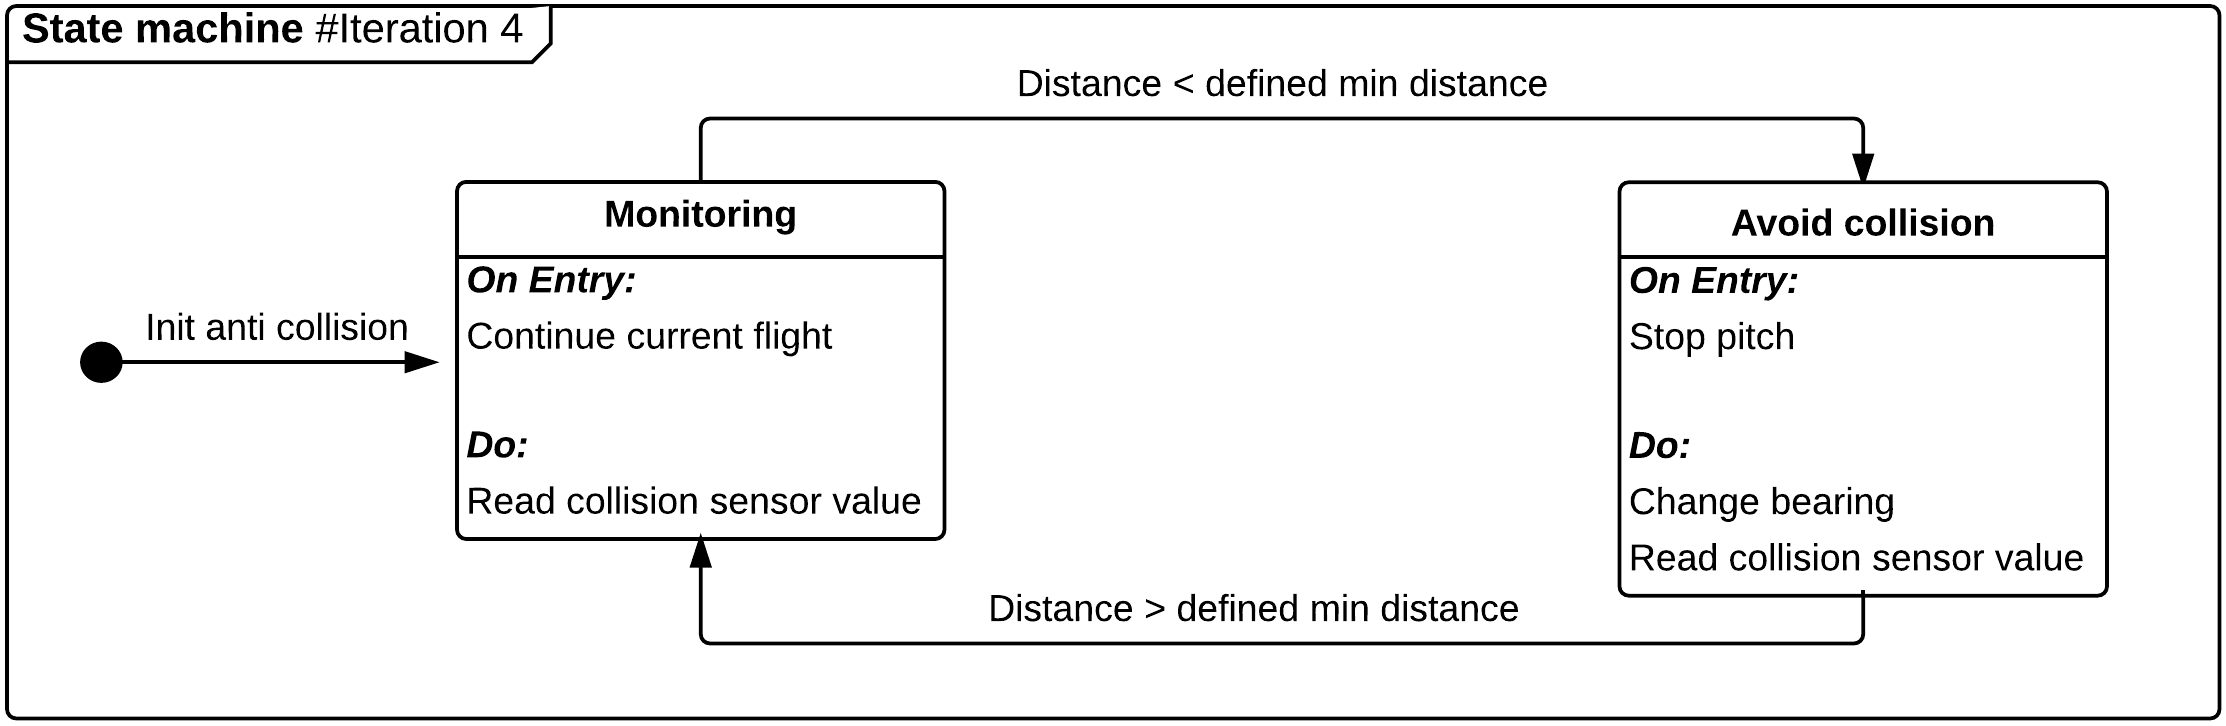
\includegraphics[width=1\textwidth]{Billeder/statemachine/State_iteration4.png}
	\vspace{-0.5cm}
	\caption{Statemachine \#iteration 4}
	\label{fig:Statemachine_iteration4}
\end{figure}